\chapter{Android Studio}

\section{Installation}
Android studio er gratis og kan installeres på Windows, Mac og Linux.\\
Man kan google Android Studio eller følge dette link:\\
\url{https://developer.android.com/studio/index.html}

På deres hjemmeside har de guides og videoer som kan hjælpe dig.
Først downloader du Android Studio og åbner derefter den hentede fil.

\section{Oprettelse af projekter}
Efter du har installeret Android Studio, åbner du det og hvis du ikke har et projekt åben kommer du til velkomst menuen, der trykker du new project.

Så skal du skrive hvad din app skal hedde, dit domaine(ikke så vigtigt hvis du ikke vil sælge den) og hvor appen skal ligge på din computer. I eksemplet har jeg valgt Min Clicker app og valgt at den skal ligge i mappen Clickerapp. 
\begin{figure}[h]
	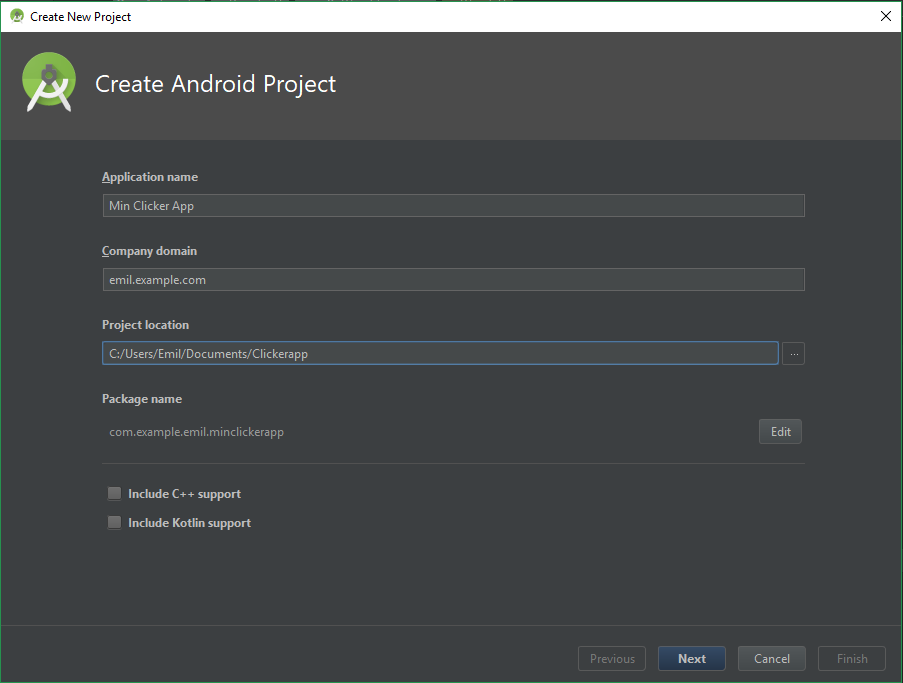
\includegraphics[width=\textwidth]{CreateProject}
	\caption{Eksempel 1.1}
	\label{fig:createproject}
\end{figure}
Det er godt at lave en mappe til sit projekt så man let kan finde det igen. 

Bagefter skal man vælge hvorfor en version af Android den laveste version skal kunne installeres på. Man kan også lave til andre platforme men det vil jeg ikke komme længere ind på. 
\begin{figure}[h]
	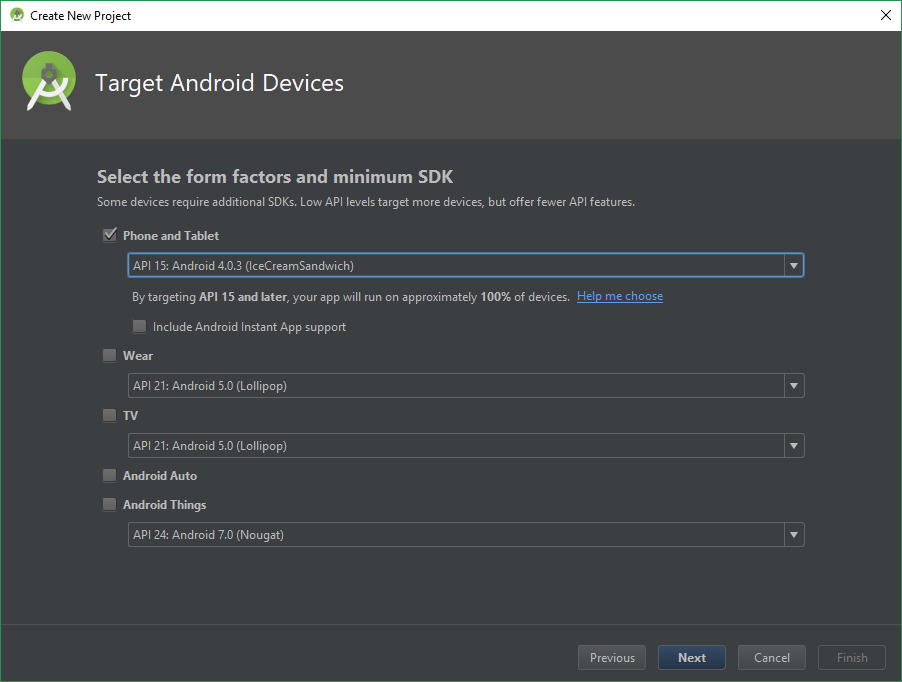
\includegraphics[width=\textwidth]{API}
	\caption{Eksempel 1.2}
	\label{fig:API}
\end{figure}

Derefter skal man vælge en Activity
Man kan vælge en pre-defineret Activity med noget funktionalitet, eller bare tage en hel tom Activity som jeg har gjort i eksemplet.

\begin{figure}[h]
	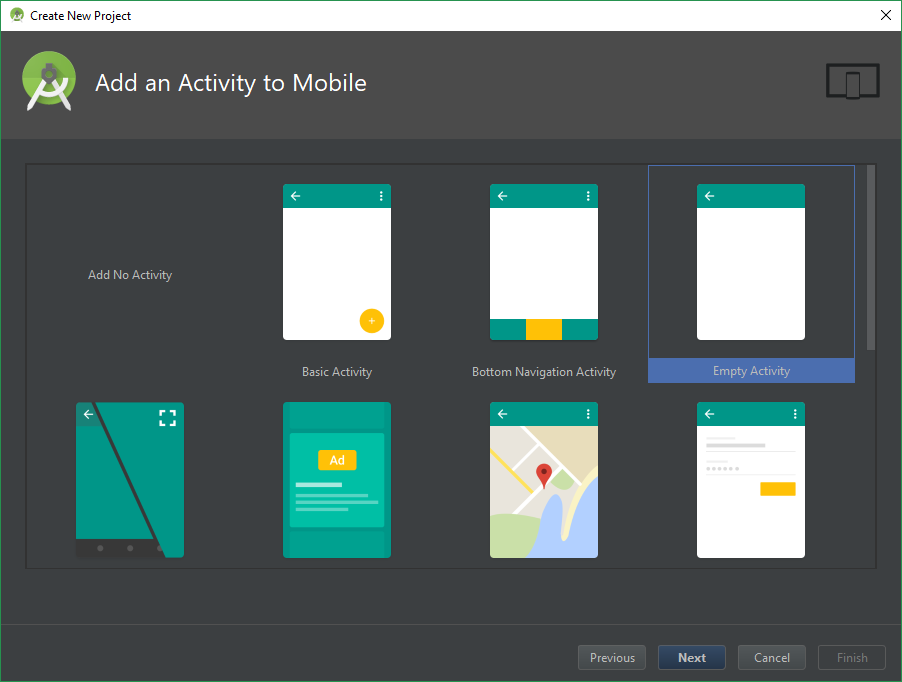
\includegraphics[width=\textwidth]{Activity}
	\caption{Eksempel 1.2}
	\label{fig:Activiy}
\end{figure}

Så skal du navngive din activity, lettest bare lade stå main activitet 

\begin{figure}[h]
	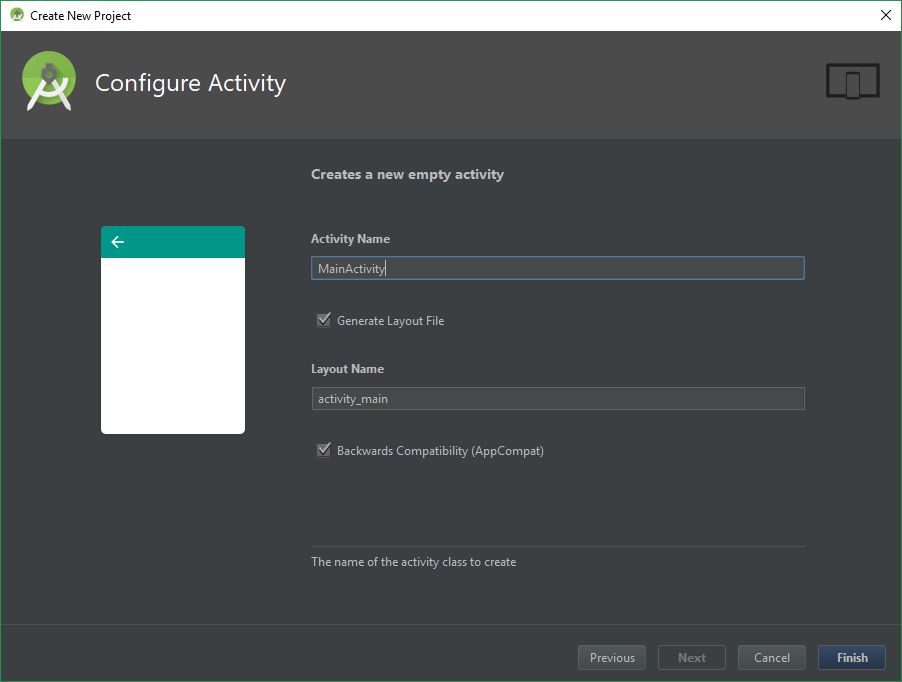
\includegraphics[width=\textwidth]{ConfigActivity}
	\caption{Eksempel 1.2}
	\label{fig:Config Activiy}
\end{figure}

Nu vil Android Studio så sætte basis tingene op.

\FloatBarrier

\section{Eksempel på udvikling af en meget simpel clicker app}

Nu da vi har fået lavet skelettet til appen skal vi have knapper og text felter

\begin{figure}[h]
	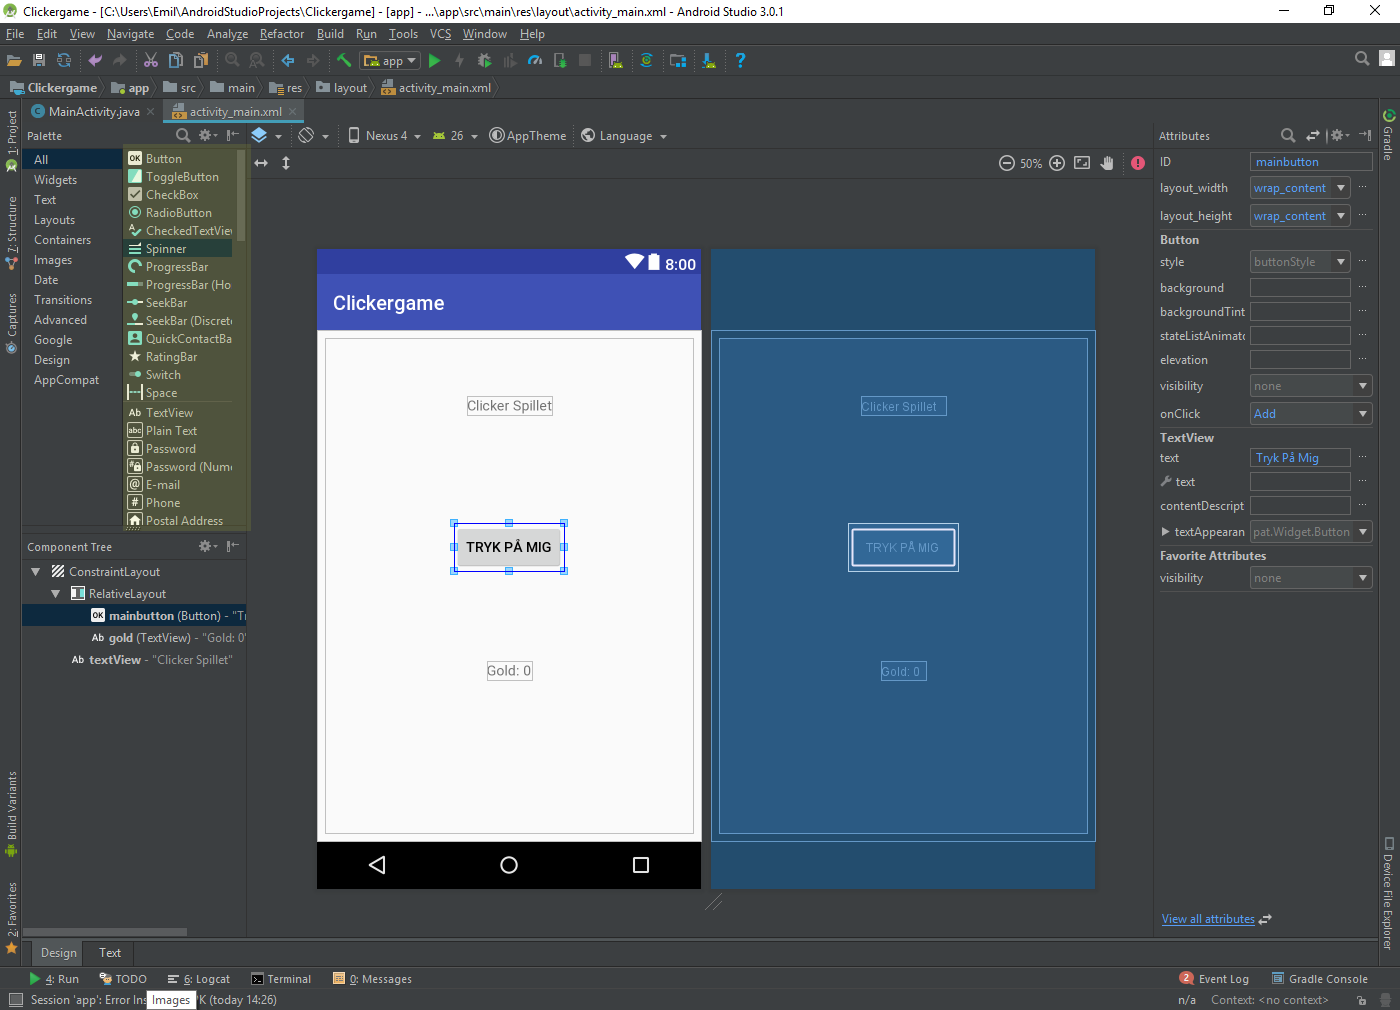
\includegraphics[width=\textwidth]{App}
	\caption{Eksempel 1.1}
	\label{fig:App}
\end{figure}

De findes i paletten som er markeret med gul. 

Tryp på Mig firkanten er en Button og Gold: 0 er et Textview. 
Knapperne og tekst felterne kan ses i component tree i venstre hjørne og der kan du også se hvis du har andre komponenter.

Hvis du har en knap eller et tekstfelt markeret kan du set dets attributes i højre side.

Det er vigtigt at hver knap eller tekst felt har et ID, så det kan findes i koden. Ellers kan du bare rode rundt med de andre. 

Der skulle også være lavet en Mainactivity java fil.

Det her er hvad jeg har skrevet i min activity. 
\begin{figure}[h]
	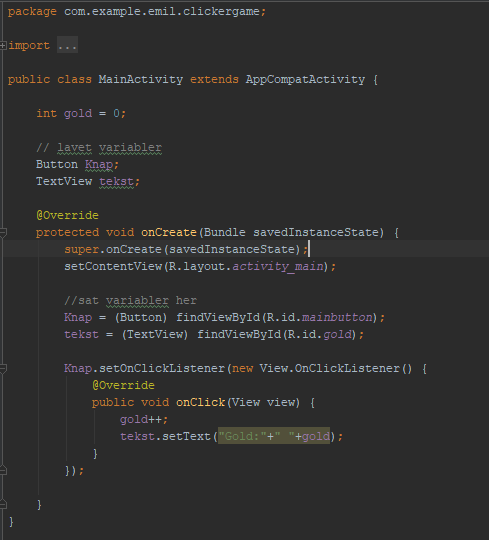
\includegraphics[width=\textwidth]{Java}
	\caption{Eksempel 1.1}
	\label{fig:Java}
\end{figure}

\begin{JavaCode}{2}{a}
	public class MainActivity extends AppCompatActivity {
		int gold = 0;
		
		Button button;
		TextView textView;
		
		@Override
		protected void onCreate(Bundle savedInstanceState) {
			super.onCreate(savedInstanceState);
			setContentView(R.layout.activity_main);
			
			button = (Button) findViewById(R.id.mainbutton);
			textView = (TextView) findViewById(R.id.gold);
			
			button.setOnClickListener(new View.OnClickListener() {
				@Override
				public void onClick(View view) {
					gold++;
					textView.setText("Gold: " + gold);	
				}
			});
		}
	}
\end{JavaCode}

Jeg har sat en variabel gold som har styr på guld beholdningen. 

Derefter har jeg lavet de to variabler Knap og tekst. 

på oncreate, som er når appen starter, har jeg sat den til at finde Knappen og tekst feltet som jeg satte ind. 

Derefter har man brug for en onclicklistener, som opfanger når folk trykker på knappen. 

Så det der sker når folk trykker på knappen er at gold øges med 1 og tekst feltet ændres til Gold og derefter hvor meget huld man har. 

Tilsidst kan appen afprøves på en android mobil eller på en emulator. på mobilen er man nød til at slå filoverførsel til. 






